\section{Fundamentos Teóricos}

\subsection{¿Qué es una curva elíptica?}

La criptografía en general nos ha acostumbrado a pensar que la seguridad se debe basar en un simple juego aritmético, pero este estándar de las curvas elípticas nos muestra que también podemos hacer criptografía con geometría. 

Una curva elíptica es un conjunto de puntos que satisfacen la ecuación en forma normal de Weierstrass $y^2 = x^3 + ax + b$ cuyo discriminante $4a^3 + 27b^2$ debe ser distinto de cero para evitar singularidades (curvas con auto-intersecciones o cúspides) e incluye además un elemento teórico indispensable llamado punto en el infinito (denotado como $0$).

\begin{definition} Curva elíptica. $$\left\{ (x, y) \in \mathbb{R}^2 \mid y^2 = x^3 + ax + b, \ 4a^3 + 27b^2 \neq 0 \right\} \cup \{0\}$$
\end{definition}

Pero si no hay una operación, no podemos hacer nada con la curva o con sus puntos. Por eso definimos la operación de suma así:

\begin{definition}
\textbf{Si trazamos una línea recta y cruza tres puntos de la curva ($P$, $Q$ y $R$), su suma es cero ($P + Q + R = 0$).}
\end{definition}

Esta definición geométrica de suma tiene la bondad de que convierte a los puntos de la curva en un grupo abeliano, con lo cual emergen muchas propiedades útiles, como la unicidad del elemento neutro o del elemento inverso aditivo. Pero nuestra definición es ternaria. Necesitamos hacerla más operativa.

Para sumar $P + Q$, se traza una línea entre ambos, se encuentra el tercer punto de intersección $R$ en la curva y se toma su reflejo sobre el eje X (es decir, $-R$). Por lo tanto, $P + Q = -R$. 

\begin{figure}[H]
    \centering
    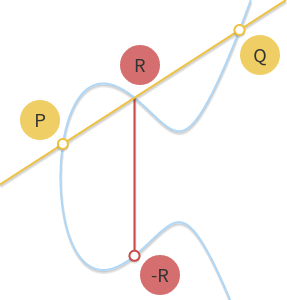
\includegraphics[width=0.5\textwidth]{imagenes/suma_cuerpo_reales.png}
    \caption{Operación geométrica de la suma  $P + Q = -R$, con puntos $P$, $Q$ y $R$ colineales en una curva elíptica sobre los reales.}
    \label{fig:suma_cuerpo_reales}
\end{figure}

Al pasar esto al álgebra, la suma requiere calcular la pendiente de la recta ($m$) entre los puntos para encontrar las coordenadas exactas del nuevo punto.

Si $P$ y $Q$ son distintos ($x_P \neq x_Q$), la línea tiene pendiente:

$$m = \frac{y_P - y_Q}{x_P - x_Q}$$


Si, por el contrario, $P$ y $Q$ son iguales, la pendiente se debe calcular de otra manera. La línea se ve como una tangente a la curva en este punto. Si queremos calcular la pendiente de una tangente, derivamos la ecuación de la curva en ese punto. Nos queda la siguiente expresión:

$$m = \frac{3x_P^2 + a}{2y_P}$$

En cualqueir caso, la intersección entre la línea y esta curva es un tercer punto: $R = (x_R, y_R)$:

$$
\begin{aligned}
x_R &= m^2 - x_P - x_Q \\
y_R &= y_P + m(x_R - x_P) = y_Q + m(x_R - x_Q)
\end{aligned}
$$

De esta manera, $(x_P, y_P) + (x_Q, y_Q) = (x_R, -y_R)$ (recordemos $P + Q = -R$).

\subsection{¿Podemos hacer criptografía con estas curvas elípticas?}

La respuesta corta: \textbf{no}. Más adelante veremos que necesitamos efectuar la operación de suma cientos de veces iterativamente. Si bien sobre el papel tienen propiedades muy intersantes, si trabajamos sobre el cuerpo de los números reales, el error propagado sobre puntos de la curva calculados se haría enorme y no sería un método confiable. 

Para usar las curvas en criptografía, debemos abandonar el conjunto de los números reales y definir la curva elíptica sobre un cuerpo finito de enteros módulo un número primo.

\begin{definition} Curva elíptica sobre cuerpo finito $\mathbb{F}_p$.
$$\{ (x, y) \in (\mathbb{F}_p)^2 \mid y^2 \equiv x^3 + ax + b \pmod p, 4a^3 + 27b^2 \not\equiv 0 \pmod p \} \cup \{0\}$$
\end{definition}

Esto tiene varias consecuencias:
\begin{itemize}
    \item La curva se vuelve un conjunto de puntos discretos representados por $y^2 \equiv x^3 + ax + b \pmod{p}$.
    \item Es necesario redefinir qué entendemos por puntos colineales.
    \item Las ecuaciones algebraicas para sumar puntos siguen siendo exactamente las mismas, pero todas las operaciones aritméticas (suma, resta, multiplicación) se calculan con el módulo $p$.
    \item La ``división'' en un cuerpo finito requiere encontrar el inverso multiplicativo mediante el algoritmo de Euclides extendido.
\end{itemize}

Es importante notar una propiedad fundamental de la aritmética modular en este paso: la operación de ``división'' (es decir, multiplicar por el inverso multiplicativo $(x_P - x_Q)^{-1} \bmod p$) solo está matemáticamente definida si el denominador $(x_P - x_Q)$ y el módulo $p$ son coprimos. Dado que en la criptografía de curvas elípticas $p$ se elige siempre como un número primo, esta condición de coprimalidad está garantizada para cualquier diferencia temporal, salvo cuando el denominador se anula por completo (es decir, cuando $x_P = x_Q$). Es en ese escenario exacto donde la fórmula de la recta secante deja de ser válida y el álgebra nos obliga, de forma natural, a transicionar a la fórmula de la pendiente de la recta tangente.

\begin{figure}[H]
    \centering
    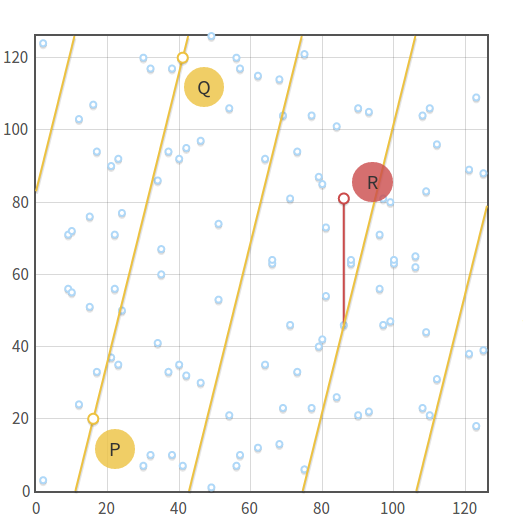
\includegraphics[width=0.5\textwidth]{imagenes/suma_cuerpo_finito.png}
    \caption[Suma de puntos sobre la curva en cuerpo finito]{Suma de puntos sobre la curva $y^2 \equiv x^3 - x + 3 \pmod{127}$, con $P = (16, 20)$ y $Q = (41, 120)$. Nótese que la línea $y \equiv 4x + 83 \pmod{127}$ que conecta los puntos se repite en el plano.}
    \label{fig:suma_cuerpo_finito}
\end{figure}

Entonces, dados los puntos colineales $P = (x_P, y_P)$, $Q = (x_Q, y_Q)$ y $R = (x_R, y_R)$, calculamos $P + Q = -R$ así:

Si $P \neq Q$, la pendiente $m$ se calcula como:

$$m = (y_P - y_Q)(x_P - x_Q)^{-1} \bmod p$$

De lo contrario, si $P = Q$, la pendiente se calcula así:

$$m = (3x_P^2 + a)(2y_P)^{-1} \bmod p$$

Y usamos este resultado en las nuevas expresiones modulares:

$$\begin{aligned}
x_R &= (m^2 - x_P - x_Q) \bmod p \\
y_R &= [y_P + m(x_R - x_P)] \bmod p \\
&= [y_Q + m(x_R - x_Q)] \bmod p
\end{aligned}$$

Y es así que finalmente calculamos:

$$P + Q = -R = (x_R, -y_R \bmod p)$$

\subsection{¿Hay algún orden en este aparente caos?}

Si sumamos puntos en $\mathbb{F}_p$, los resultados saltan por todo el plano de forma aparentemente caótica. ¿Cómo confiamos en algo caótico?

Saber que una curva elíptica sobre un cuerpo finito $\mathbb{F}_p$ forma un grupo abeliano bajo la operación de suma de puntos no es suficiente para garantizar la viabilidad de un protocolo; necesitamos conocer la topología exacta de este grupo, denotado como $E(\mathbb{F}_p)$. Es aquí donde interviene una pieza clave del álgebra abstracta.

\begin{theorem} Teorema Fundamental de los Grupos Abelianos Finitos.
Todo grupo abeliano finito es isomorfo a un producto directo de grupos cíclicos cuyos órdenes son potencias de números primos.
\end{theorem}

Al aplicar este teorema a la teoría de curvas algebraicas, obtenemos un resultado maravillosamente restrictivo y preciso. Nos garantiza que el grupo de puntos $E(\mathbb{F}_p)$ es isomorfo a, como máximo, el producto de dos grupos cíclicos:

$$E(\mathbb{F}_p) \cong \mathbb{Z}_{q_1} \times \mathbb{Z}_{q_2}$$

Donde $q_1$ y $q_2$ son enteros positivos tales que $q_1$ divide a $q_2$, y a su vez $q_1$ divide a $p-1$. En el caso particular (y muy buscado en criptografía) donde $q_1 = 1$, la curva forma un único grupo cíclico $\mathbb{Z}_{q_2}$.

Saber que la curva se descompone matemáticamente en esta estructura fundamenta la aplicación de estándares como el GOST R 34.10 en tres aspectos críticos:

\begin{itemize}
    \item \textbf{Selección del punto generador ($P$):} Para hacer criptografía, requerimos un punto base $P$ que, al someterse a multiplicación escalar sucesiva, genere una trayectoria predecible y extensa antes de alcanzar el punto en el infinito ($0$). El teorema nos asegura la existencia de un generador para un subgrupo cíclico de orden estricto $q$.
    \item \textbf{Base del Logaritmo Discreto:} La seguridad de los protocolos de firma digital no opera sobre la totalidad de los puntos de la curva, sino confinada dentro de un subgrupo cíclico principal. El teorema garantiza matemáticamente la existencia y la delimitación de estos subgrupos.
    \item \textbf{Evasión de vulnerabilidades:} Conocer la descomposición en $\mathbb{Z}_{q_1} \times \mathbb{Z}_{q_2}$ permite auditar la curva. Si el orden del subgrupo cíclico ($q$) se llegara a factorizar en números primos pequeños, algoritmos como el de Pohlig-Hellman podrían quebrar la clave reduciendo el problema a subgrupos menores. Gracias a esta certeza algebraica, los criptógrafos configuran los parámetros para asegurar que el orden $q$ sea un primo inmenso, neutralizando este vector de ataque.
\end{itemize}

\subsection{¿Cómo aplicamos las curvas elípticas a la criptografía?}

Si sumamos un punto $P$ consigo mismo $n$ veces ($nP = P + P + \dots + P$), obtenemos un nuevo punto de la curva. Esta operación llamada multiplicación escalar es la base directa de la criptografía de curva elíptica.

\begin{definition} Multiplicación escalar.
$$nP = \underbrace{P + P + \dots + P}_{n \text{ veces}}$$
\end{definition}

En una aplicación criptográfica seria vamos a tener un escalar $n$ de cientos de cifras. Para un escalar $n$ de $k$ bits, que es como realmente se miden estos números en criptografía, el algoritmo de sumar de uno en uno los puntos $P$ tiene una complejidad temporal $\mathcal{O}(2^k)$, inalcanzable computacionalmente. Para esto se diseñó el algoritmo de ``doblar y sumar'' (\textit{double and add}), el cual descompone $n$ en potencias de dos a partir de su representación binaria. Esto reduce drásticamente el tiempo de cómputo a una complejidad de $\mathcal{O}(k)$, volviendo la operación fácil y rápida para las computadoras.


\begin{figure}[H]
    \centering
    \begin{tikzpicture}[node distance=0.8cm and 2cm]

        % Bloques principales
        \node (start) [startstop] {Inicio \\ \small (Entrada: $n, P$)};
        
        \node (init) [process, below=of start] {\texttt{result} = 0 \\ \texttt{addend} = $P$};
        
        \node (while_cond) [decision, below=of init] {¿Quedan bits \\ en $n$?};
        
        % Eliminamos el \& problemático usando \texttt
        \node (get_bit) [process, below=of while_cond] {\texttt{bit} = \texttt{least\_significant\_bit(n)} \\ n = \texttt{right\_shift(n)}};
        
        \node (check_bit) [decision, below=of get_bit] {¿\texttt{bit} == 1?};
        
        \node (add_step) [process, below=of check_bit] {\texttt{result} += \texttt{addend}};
        
        \node (double_step) [process, below=1.2cm of add_step] {\texttt{addend} *= 2};
        
        \node (stop) [startstop, right=of while_cond] {Fin \\ \small (Retorna \texttt{result})};

        % Conexiones y flujos
        \draw [arrow] (start) -- (init);
        \draw [arrow] (init) -- (while_cond);
        
        % De la condición del bucle (While)
        \draw [arrow] (while_cond) -- node[anchor=east] {Sí} (get_bit);
        \draw [arrow] (while_cond) -- node[anchor=south] {No} (stop);
        
        \draw [arrow] (get_bit) -- (check_bit);
        
        % Condicional del bit (If bit == 1)
        \draw [arrow] (check_bit) -- node[anchor=east] {Sí} (add_step);
        \draw [arrow] (add_step) -- (double_step);
        
        % Camino "No" del condicional del bit
        \draw [arrow] (check_bit.west) -- node[anchor=south] {No} ++(-1.5cm,0) |- (double_step.west);
        
        % Retroalimentación del bucle (Regresar a evaluar la condición)
        \draw [arrow] (double_step.east) -- ++(2cm,0) |- (while_cond.south east);

    \end{tikzpicture}
    \caption{Diagrama de flujo del algoritmo \textit{Double and Add}.}
    \label{fig:double_and_add}
\end{figure}

Al multiplicar un punto base $P$ repetidas veces sobre un cuerpo finito, los resultados no cubren toda la curva, sino que forman un subgrupo cíclico que se repite infinitamente (por ejemplo: $P, 2P, 3P, 4P, 0$).
\begin{itemize}
    \item \textbf{Orden del subgrupo ($n$):} Es la cantidad de puntos que tiene el ciclo y equivale al menor número $n$ para el cual $nP = 0$.
    \item \textbf{Teorema de Lagrange:} Establece que el orden de este subgrupo ($n$) siempre debe ser un divisor exacto del orden total de puntos que tiene la curva elíptica completa ($N$).
    \item \textbf{Cofactor ($h$):} Es el resultado de dividir el orden total de la curva entre el orden del subgrupo ($h = N / n$). En criptografía, se busca que $n$ sea un número primo muy grande y se usa el cofactor para encontrar un punto generador ($G$) seguro multiplicando un punto aleatorio $P$ por $h$ ($G = hP$).
\end{itemize}

Si bien calcular la múltiplicación escalar para un $n$ elevado es fácil, el problema inverso de encontrar $n$ sabiendo $P$ y $nP$ es extremadamente difícil. Este es llamado el Problema del Logaritmo Discreto (DLP), y es el corazón de la seguridad del sistema. 

\begin{definition} Problema del Logaritmo Discreto (DLP).
Si conocemos un punto base $P$ y otro punto $Q$ en una curva elíptica sobre $\mathbb{F}_p$, ¿cuál es el número $n$ tal que $Q = nP$? \\
\end{definition}

Debido a que la multiplicación escalar sobre cuerpos finitos parece caótica y da saltos discretos impredecibles en el plano, resolver este Problema del logaritmo discreto es computacionalmente ``difícil''. No existe ningún algoritmo de tiempo polinómico para computadoras clásicas que pueda encontrar el número secreto $n$ fácilmente. Esta asimetría matemática (fácil de multiplicar, inviable de revertir) es lo que garantiza que la clave privada permanezca segura.

El estándar criptográfico ruso GOST R 34.10-2012 se apoya exactamente en esta fundamentación matemática, operando sobre curvas elípticas en forma de Weierstrass con cuerpos finitos primos de $256$ o $512$ bits. Los parámetros de la curva (como $a$, $b$, el primo $p$ y el generador $P$) están estrictamente definidos por el estándar para garantizar que el cofactor $h$ sea óptimo y evite subgrupos débiles.